\documentclass{beamer}

\usepackage[utf8]{inputenc}
\usepackage{default}


\usepackage{multirow} %for aligning stuff in tables

\usepackage{bbding} %for the smiley face

\usepackage{calc} %calculate spacing \widthof

%tikz stuff
\usepackage{tikzsymbols}
\usepackage{tikz}
\usetikzlibrary{fit,arrows,positioning}

  % Keys to support piece-wise uncovering of elements in TikZ pictures:
  % \node[visible on=<2->](foo){Foo}
  % \node[visible on=<{2,4}>](bar){Bar}   % put braces around comma expressions
  %
  % Internally works by setting opacity=0 when invisible, which has the
  % adavantage (compared to \node<2->(foo){Foo} that the node is always there, hence
  % always consumes space plus that coordinate (foo) is always available.
  %
  % The actual command that implements the invisibility can be overriden
  % by altering the style invisible. For instance \tikzsset{invisible/.style={opacity=0.2}}
  % would dim the "invisible" parts. Alternatively, the color might be set to white, if the
  % output driver does not support transparencies (e.g., PS)
  %
  \tikzset{
    invisible/.style={opacity=0},
    visible on/.style={alt={#1{}{invisible}}},
    alt/.code args={<#1>#2#3}{%
      \alt<#1>{\pgfkeysalso{#2}}{\pgfkeysalso{#3}} % \pgfkeysalso doesn't change the path
    },
  }
  \tikzset{
    dimmed/.style={opacity=0.2},
    dimmed on/.style={alt={#1{dimmed}{}}},
    alt/.code args={<#1>#2#3}{%
      \alt<#1>{\pgfkeysalso{#2}}{\pgfkeysalso{#3}} % \pgfkeysalso doesn't change the path
    },
  }
\tikzset{
    %Define standard arrow tip
    >=stealth',
    %Define style for boxes
    peer/.style={
           rectangle,
           rounded corners,
           draw=black, thin,
           text width=3.5em,
           minimum height=2em,
           text centered},
    node/.style={
           rectangle,
           rounded corners,
           draw=black,
           text width=4.5em,
           minimum height=2em,
           text centered,
           fill={rgb:black,1;white,3}},
    chunk/.style={
           rectangle,
           rounded corners,
           draw=black,
           text width=2.5em,
           minimum height=1em,
           text centered,
           fill=block title bg},
    % Define arrow style
    point/.style={
           ->,
           thick,
           shorten <=2pt,
           shorten >=2pt,}
every node/.style={align=center}
}

\newcommand{\wholeslide}[2][]{
\begin{frame}{#1}
% \transboxout<1>[duration=0.5]
\setbeamercolor{bgcolor}{fg=black,bg=white}
\begin{tikzpicture}[overlay, remember picture]
\node[anchor=center] at (current page.center) {
  \begin{beamercolorbox}[center]{bgcolor}
     #2
  \end{beamercolorbox}};
\end{tikzpicture}

\end{frame}
}

\newcommand{\blankslide}[2][]{
\begin{frame}[plain]{#1}
% \transboxout<1>[duration=0.5]
\setbeamercolor{bgcolor}{fg=black,bg=white}
\begin{tikzpicture}[overlay, remember picture]
\node[anchor=center] at (current page.center) {
  \begin{beamercolorbox}[center]{bgcolor}
     #2
  \end{beamercolorbox}};
\end{tikzpicture}

\end{frame}
}

\newenvironment<>{varblock}[2][.9\textwidth]{%
  \setlength{\textwidth}{#1}
  \begin{actionenv}#3%
    \def\insertblocktitle{#2}%
    \par%
    \usebeamertemplate{block begin}}
  {\par%
    \usebeamertemplate{block end}%
  \end{actionenv}}

\newlength{\mywidth}
\newcommand{\blockslide}[3][]{
\settowidth{\mywidth}{#3}
\begin{frame}[c]{#1}
\begin{center}
\begin{minipage}{1.1\mywidth}
 \begin{varblock}[1.1\mywidth]{#2}
  #3
 \end{varblock}
\end{minipage}
\end{center}
\end{frame}
}


\newcommand{\plainblockslide}[2]{
\settowidth{\mywidth}{#2}
\begin{frame}[c]
\begin{center}
\begin{minipage}{1.1\mywidth}
 \begin{varblock}[1.1\mywidth]{#1}
  #2
 \end{varblock}
\end{minipage}
\end{center}
\end{frame}
}

\mode<presentation>{
\usetheme{Warsaw}\usecolortheme{crane}
\setbeamertemplate{items}[square]
\setbeamertemplate{section in toc}[square]
\setbeamertemplate{subsection in toc}[square]
% \setbeamertemplate{subsection in toc}[subsections numbered]
\setbeamertemplate{subsubsection in toc}[square]
% \setbeamercolor{items}{fg=black,bg=yellow}
\usebeamercolor{block title}
\definecolor{block title bg}{named}{bg}
\setbeamercolor{item projected}{fg=black,bg=block title bg}
\setbeamercolor{itemize item}{fg=block title bg,bg=block title bg}
}






\title{swap, swear and swindle games}
\author{Viktor Trón}
% \date{Ethereum London Meetup \today}

\AtBeginSection[]
{
\begin{frame}<beamer>
\frametitle{outline}
\tableofcontents[currentsection,sectionstyle=show/shaded,subsectionstyle=show/show/hide,subsubsectionstyle=show/show/show/hide]
\end{frame}
}

\begin{document}

\begin{frame}
 \titlepage
\end{frame}


\section{status}


\subsection[swarm]{swarm: properties and services}


 \begin{frame}{swarm}
 \begin{block}{}
 storage for web3: archival and retrieval monetized
 \end{block}
 \begin{block}{}
 serving web applications with routed messaging
 \end{block}
 \begin{block}{}
 silly world of acronyms, riddles and mnemonics
 \end{block}
 \end{frame}


\begin{frame}{swarm:  properties}
\begin{block}{}
  zero downtime
\end{block}
\begin{block}{}
  fault tolerance
\end{block}
\begin{block}{}
  censorship resistance
\end{block}
\begin{block}{}
  self-sustaining
\end{block}
\begin{block}{}
  auto-scaling
\end{block}
\end{frame}

\begin{frame}{swarm: services}
\begin{block}{}
  document storage
\end{block}
\begin{block}{}
  content distribution
\end{block}
\begin{block}{}
  virtual hosting
\end{block}
\begin{block}{}
  internode messaging
\end{block}
\begin{block}{}
  decentralised database services
\end{block}
\begin{block}{}
  payments and service guarantees
\end{block}
\end{frame}

%
\begin{frame}{features and implementation}
\begin{overlayarea}{\textwidth}{10cm}
\setbeamercovered{transparent}% Dim out "inactive" elements
\begin{columns}[t]
  \column{0.5\textwidth}
    \begin{block}<1->{Feature}
      \begin{enumerate}
       \item<2,7> \textbf<2>{efficiency}
       \item<3,7> \textbf<3>{reliability}
       \item<4,7> \textbf<4>{integrity}
       \item<5,7> \textbf<5>{access and security}
       \item<5,7> \textbf<5>{domain name resultion}
       \item<6-7> \textbf<6>{attribution}
      \end{enumerate}
    \end{block}
    \begin{block}<2-6>{why?}
      \only<2>{so that all content is accessible, popular content has low latency (comp. Web2)}
      \only<3>{so that stored content does not get lost}
      \only<4>{so that there is no more hacked websites}
      \only<5>{so that only people with proper authorisation can access content}
      \only<6>{so that mutable content is reliably updated, ownership and authorship}
    \end{block}
  \column{0.5\textwidth}
    \begin{block}<2-6>{how?}
      \only<2>{
	  SWAP incentive structure: popular content is readily available\\
	  Payment-channel integration: fast and cheap
	  }
      \only<3>{
      \begin{itemize}
       \item redundant storage
       \item erasure coding
       \item storage insurance
       \item automatic scan-and-repair
      \end{itemize}
      }
      \only<4>{
      \begin{itemize}
        \item Merkle trees, binary merkle tree hash
       \item Merkle proof compatible file `manifests'
       \item chunk traversal follows Merkle-proof logic
      \end{itemize}
      }
      \only<5>{
      \begin{itemize}
        \item ecryption for privacy
        \item obfuscation for plausible deniability
        \item hierarchical keys for access control
        \item restricted access voucher exchange
        \item anonymous browsing
      \end{itemize}
      }
      \only<6>{ENS + smart contracts}
      \only<7>{
\includegraphics[width=0.3\textwidth]{swarmlogo.png} Swarm!}
    \end{block}
\end{columns}
\end{overlayarea}
\end{frame}


\begin{frame}{API-s}
\begin{overlayarea}{\textwidth}{10cm}
\begin{tikzpicture}
\node[scale=0.8] at (current page.center) {
\begin{tikzpicture}

 \node[draw,rounded corners] at (4,4) (goapi) {
\includegraphics[width=2cm]{golang.png} API};

 \node[draw,rounded corners] at (0,0) (ipc) {JSON IPC};
 \node[draw,rounded corners] at (4,0) (proxy) {http-
\includegraphics[width=1cm]{proxy.jpg}-proxy};
 \node[draw,rounded corners] at (8,0) (fuse) {fuse 
\includegraphics[width=1cm]{fuse.jpg}};

 \node[draw,rounded corners] at (2,-4) (cli) {CLI 
\includegraphics[width=1cm]{cli.png}};
 \node[draw,rounded corners] at (6,-4) (web3js) {web3.js};

 \node {}
 (cli) edge[point,->] (ipc)
 (web3js) edge[point,->] (ipc)
 (cli) edge[point,->] (proxy)
 (web3js) edge[point,->] (proxy)
 (cli) edge[point,->] (fuse)
 (web3js) edge[point,->] (fuse)
 (ipc) edge[point,->] (goapi)
 (proxy) edge[point,->] (goapi)
 (fuse) edge[point,->] (goapi)
 ;
\end{tikzpicture}
};
\end{tikzpicture}
\end{overlayarea}
\end{frame}




\subsection[roadmap]{roadmap: what's next for swarm?}

\begin{frame}
\begin{block}{POC0.3 (Q4 2017)}
 \begin{itemize}
  \item new networking layer - syncing, retrieval
  \item pss messaging
  \item network simulation framework
  \item bandwidth accounting
  \item FUSE integration
  \item light modes of operation (mobile clients)
  \item ENS support tld-specific endpoints
  \item pyramid chunker with binary merkle tree hash
  \item encryption for privacy
 \end{itemize}
\end{block}
\end{frame}

\begin{frame}
\begin{block}{POC0.4 = swarm 1.0pre (Q3 2018)}
 \begin{itemize}
  \item multicast, broadcast support
  \item obfuscation for plausible deniability
  \item multihash and mutable resource update notifications
  \item one-to-many streaming support, adaptive multibitrate codec support
  \item erasure codes with scan-and-repair service
  \item swap, swear and swindle games support
  \item proof-of-custody-based storage insurance
  \item decentalised database support (blockchain/state on swarm)
  \item provable analytics support
 \end{itemize}
\end{block}
\end{frame}

\subsection[credits]{credits and contributors}


\begin{frame}[plain]{the team}

\begin{block}{the team}
\begin{itemize}
\item Daniel A. Nagy, Zahoor Mohamed, Fabio Barone, Anton Evangelatov, Daniel A. Nagy, Viktor Trón, Zsolt Felföldi (EF core team)
\item Aron Fischer, Elad Verbin, \& Ethersphere orange lounge group
\item Lewis Marshal, Louis Holbrook, Oren Sokolowsky (Jaak)
\item Ram Devish, Bas van Kervel, Alex van der Sande, Fabian Vogensteller (EF Mist integration)
\item Felix Lange, Peter Szilagyi (EF integration, devp2p)
\item Igor Shadurin (swarm explorer dapp)
\item Nick Johnson, Alex van der Sande (Ethereum Name Service)
\item Gavin Wood, Vitalik Buterin, Jeffrey Wilcke (visionaries)
\end{itemize}
\end{block}

\end{frame}


\begin{frame}[plain]{friends}
  
\includegraphics[width=\textwidth]{friends.png}

\end{frame}

\subsection{scalable inftrastructure for web3}

\subsubsection{internode communication: pss}
\begin{frame}{pss}
\begin{block}{}
pss...  bzz + shh = whispered
\end{block}
\begin{block}{}
postal services suite
\end{block}
\begin{block}{}
p2p-protocol secure socket
\end{block}
\end{frame}
%
\subsubsection{decentralised database services}
% \begin{frame}{decentralised database services}
% \begin{block}{}
% \begin{itemize}
%   \item
%   \item provable
% \end{itemize}
% \end{block}
% \end{frame}
%
\begin{frame}{P.O.T.}
\begin{block}{self-adjusting data structure}
  optimal retrieval performance, pruning for cache
\end{block}
\begin{block}{on-disk persistance}
  garbage collection, cheap reorgs
\end{block}
\begin{block}{outsourceable updates}
  protocol for data structure updates and indexing
\end{block}
\begin{block}{typed attribute value structures}
  prove statements by verifying inclusion proofs on the blockchain
\end{block}
\begin{block}{provable indexing}
  trustless provision - decentralised db services
\end{block}

\end{frame}
%

\section{swap swear and swindle games}
% \section{}

\begin{frame}{swap swear and swindle}
\begin{block}{}
scalable base-layer infarstructure for decentralised service economies
\end{block}
\begin{block}{swap: transaction}
swarm accounting protocol
\end{block}
\begin{block}{swear: commitment}
service warranty enforcement with account registration
\end{block}
\begin{block}{swindle: enforcement}
secured with insurance, deposit, litigation and escrow
\end{block}
\end{frame}

\subsection[swap]{swap: swarm accounting protocol}
\begin{frame}{from a simple chequebook to a swap contract}
\begin{block}{swarm accounting protocol}
accounting protocol for bidirectional services
\end{block}
\begin{block}{service wanted and provided}
service for service exchange
\end{block}
\begin{block}{service with automated payments}
payment threshold reached, send a cheque
\end{block}
\begin{block}{send waiver as payment}
pay off from uncashed cheque
\end{block}
\begin{block}{set up a wallet as payment}
zero ether entry to ecosystem
\end{block}
\end{frame}

\begin{frame}{service wanted and provided}
\begin{block}{service for service}
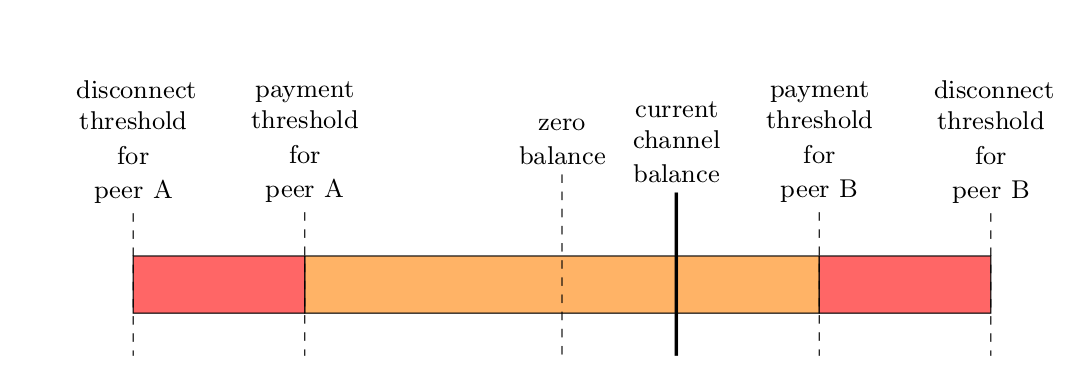
\includegraphics[width=\textwidth]{swap.png}
\end{block}
\end{frame}

\begin{frame}{settle with automated payment}
\begin{block}{sending a cheque}
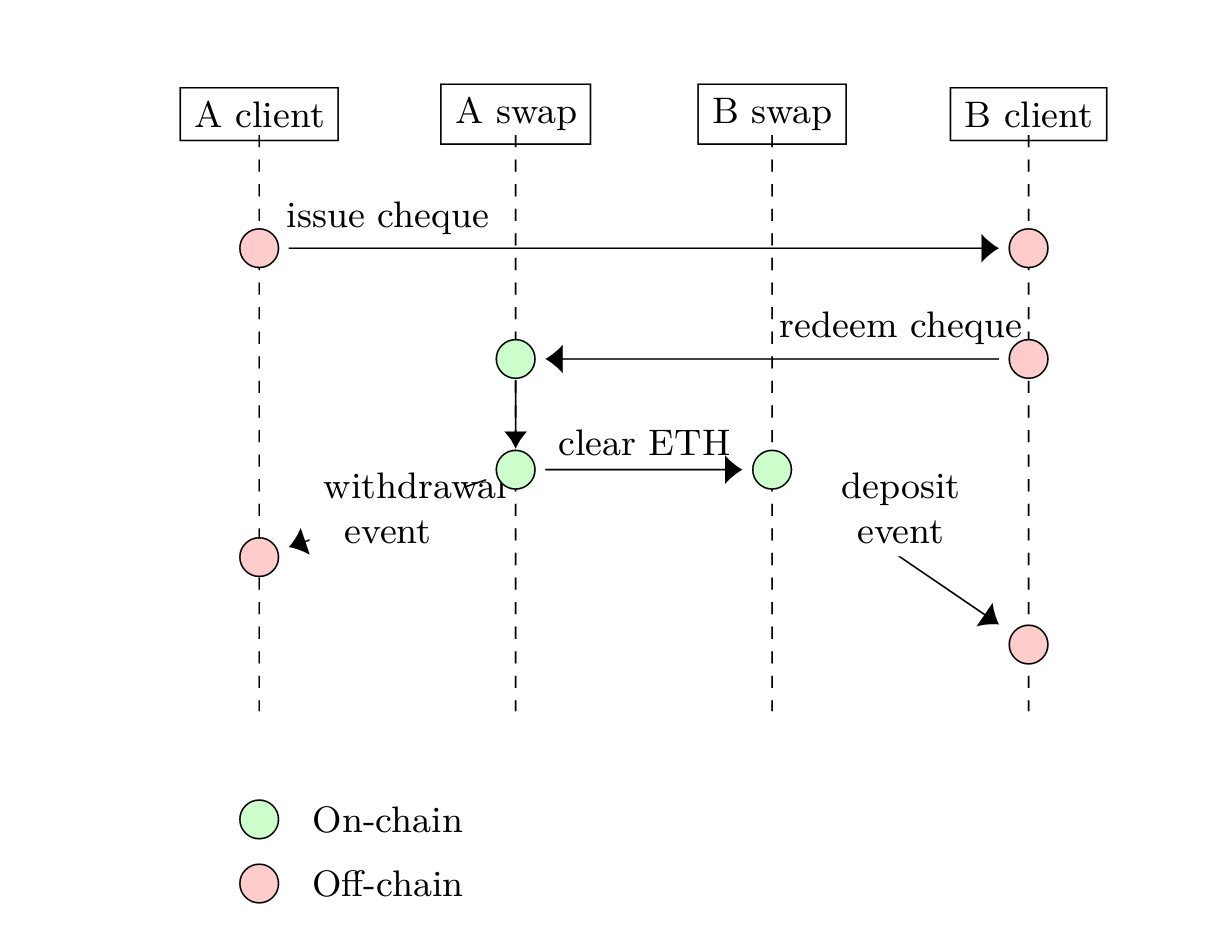
\includegraphics[width=\textwidth]{cheque-sequence.png}
\end{block}
\end{frame}

\begin{frame}{send waiver as payment}
\begin{block}{waiving an uncashed cheque}
  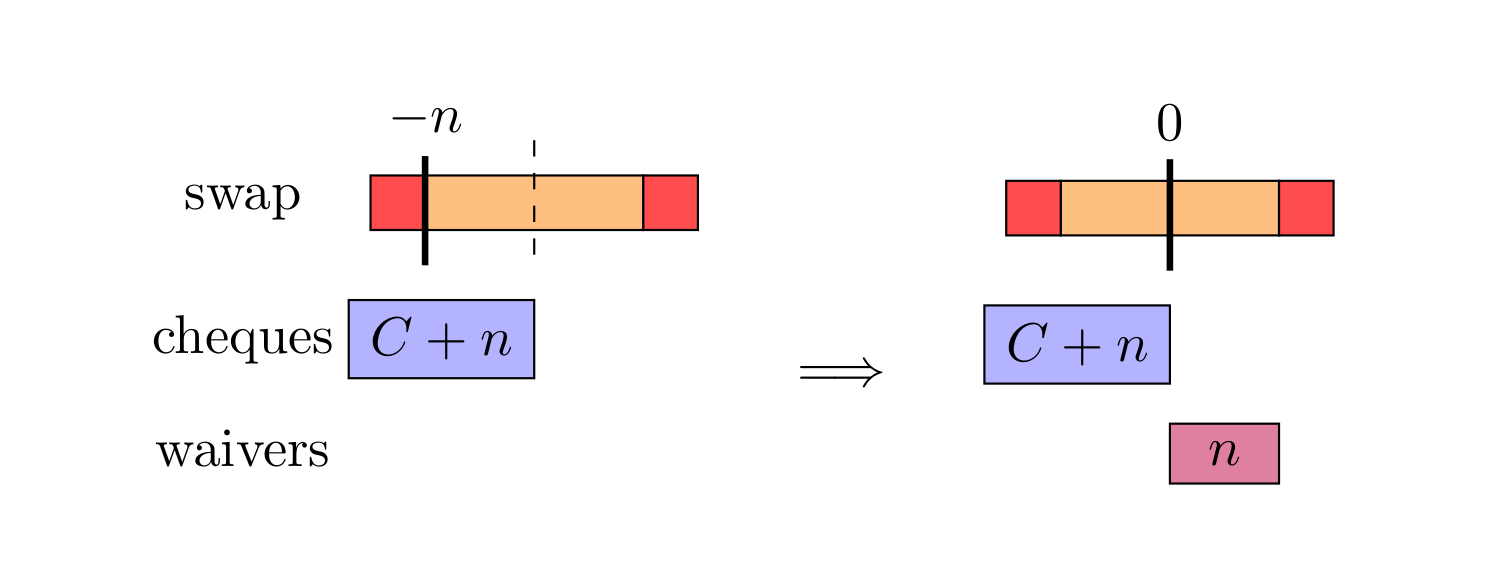
\includegraphics[width=\textwidth]{waiver.png}
\end{block}
\end{frame}


\begin{frame}{channel deposits and payment channels}
\begin{block}{balances and deposits}
  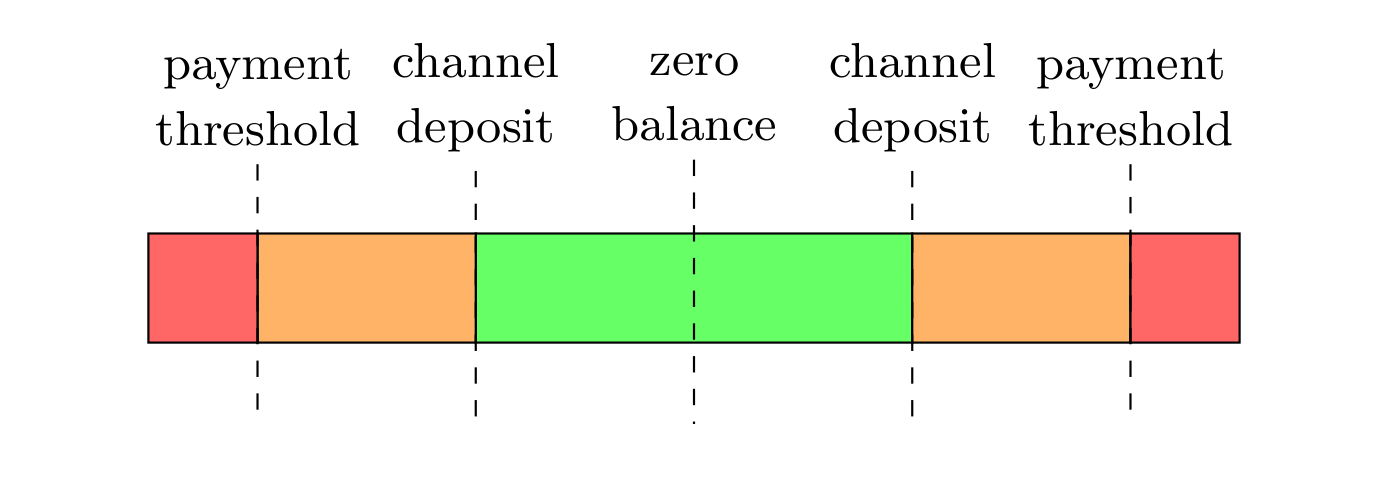
\includegraphics[width=\textwidth]{payment-channel.png}
\end{block}
\end{frame}

\begin{frame}{hard and soft channel deposits}
\begin{block}{balances and deposits}
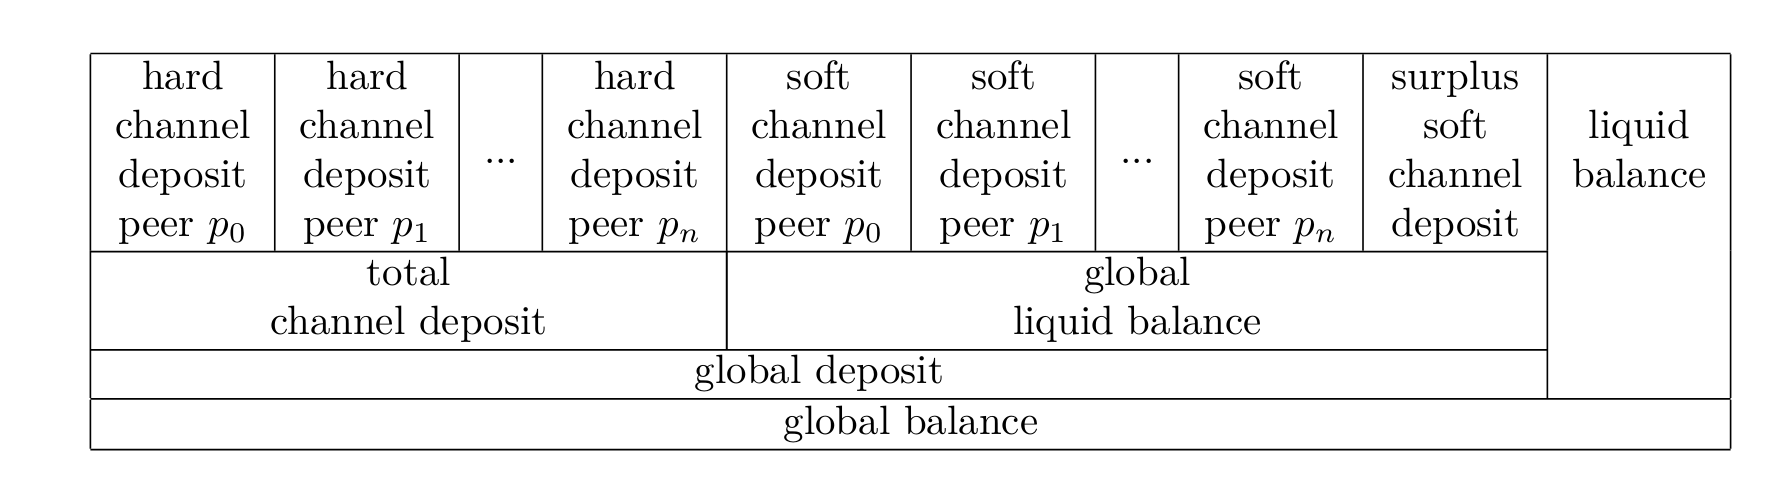
\includegraphics[width=\textwidth]{deposits.png}
\end{block}
\end{frame}


\begin{frame}{promissory notes}
\begin{block}{}
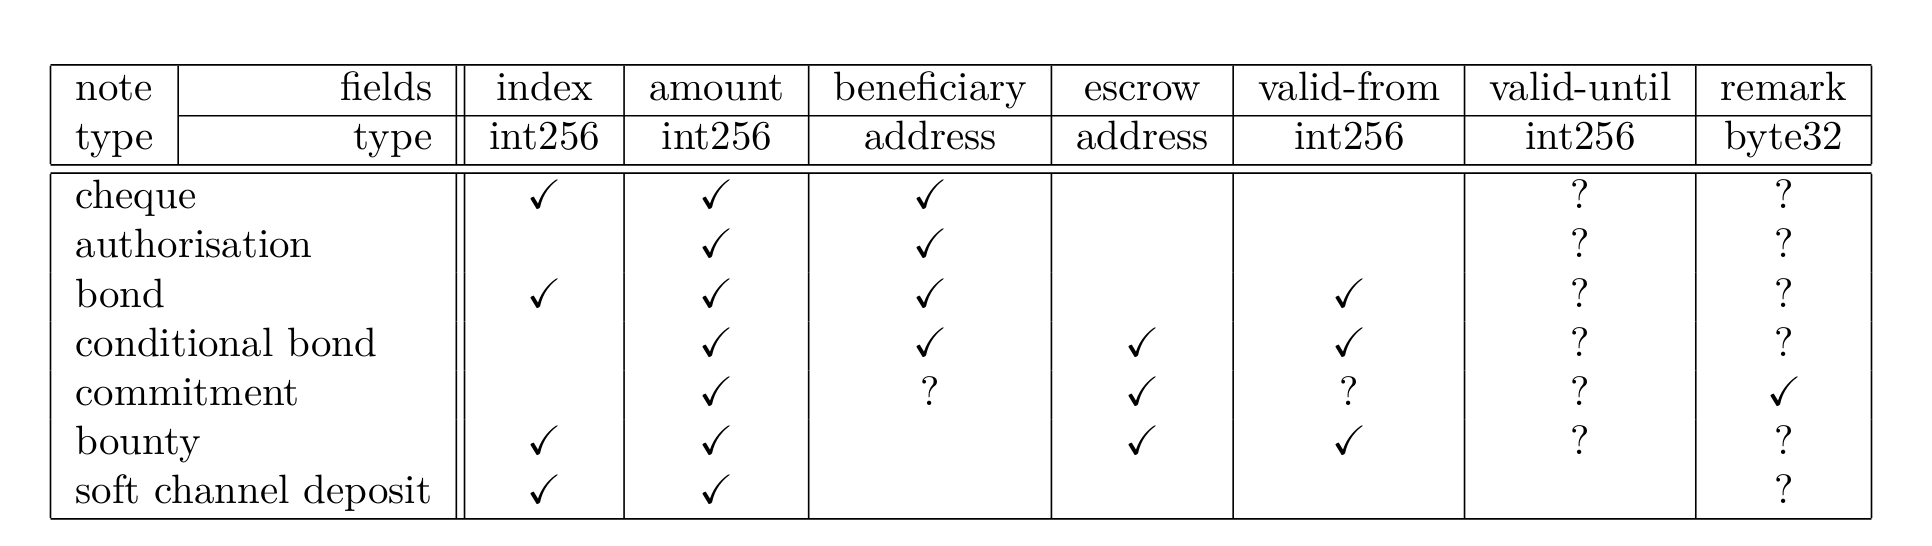
\includegraphics[width=\textwidth]{promissory-notes.png}
\end{block}
\end{frame}

\subsection[swear]{swear: service warranty, enforcement with account registration}
\begin{frame}{service guarantees}
  \begin{block}{commitment}
    provider commits to a sw3 game contract
  \end{block}
  \begin{block}{litigation}
    commitment submitted to the swap, calls swear as escrow, authorises courtroom to conduct trial
  \end{block}
  \begin{block}{enforcement}
    execute the verdict, swap authorises swear to confiscate deposit
  \end{block}
\end{frame}

\subsection[swindle]{swindle: secured with insurance, deposit, litigation and escrow}

\begin{frame}{swindle}
\begin{block}{courtroom trial}
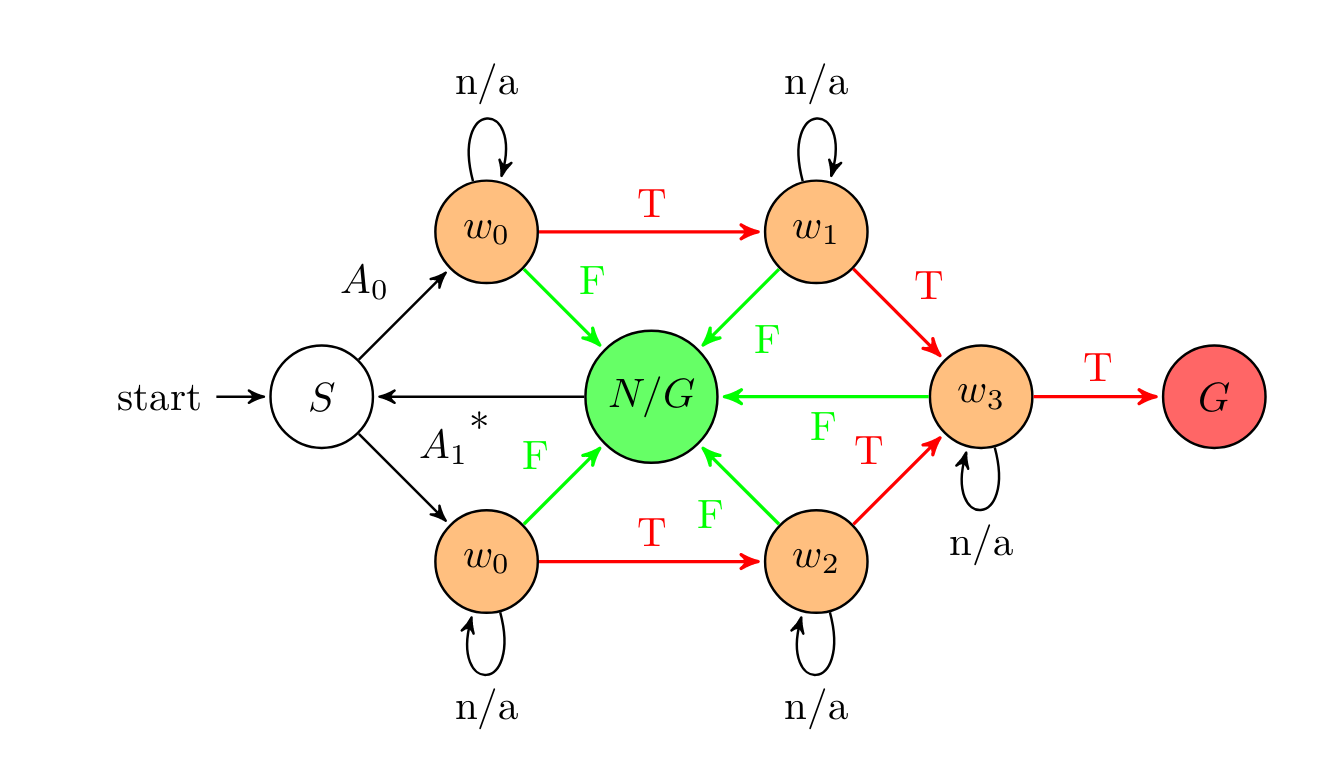
\includegraphics[width=\textwidth]{fsa-swindle.png}
\end{block}
\end{frame}


\subsection{swap channel networks}

\begin{frame}{overlay and underlay network}
\begin{block}{swap channel networks}
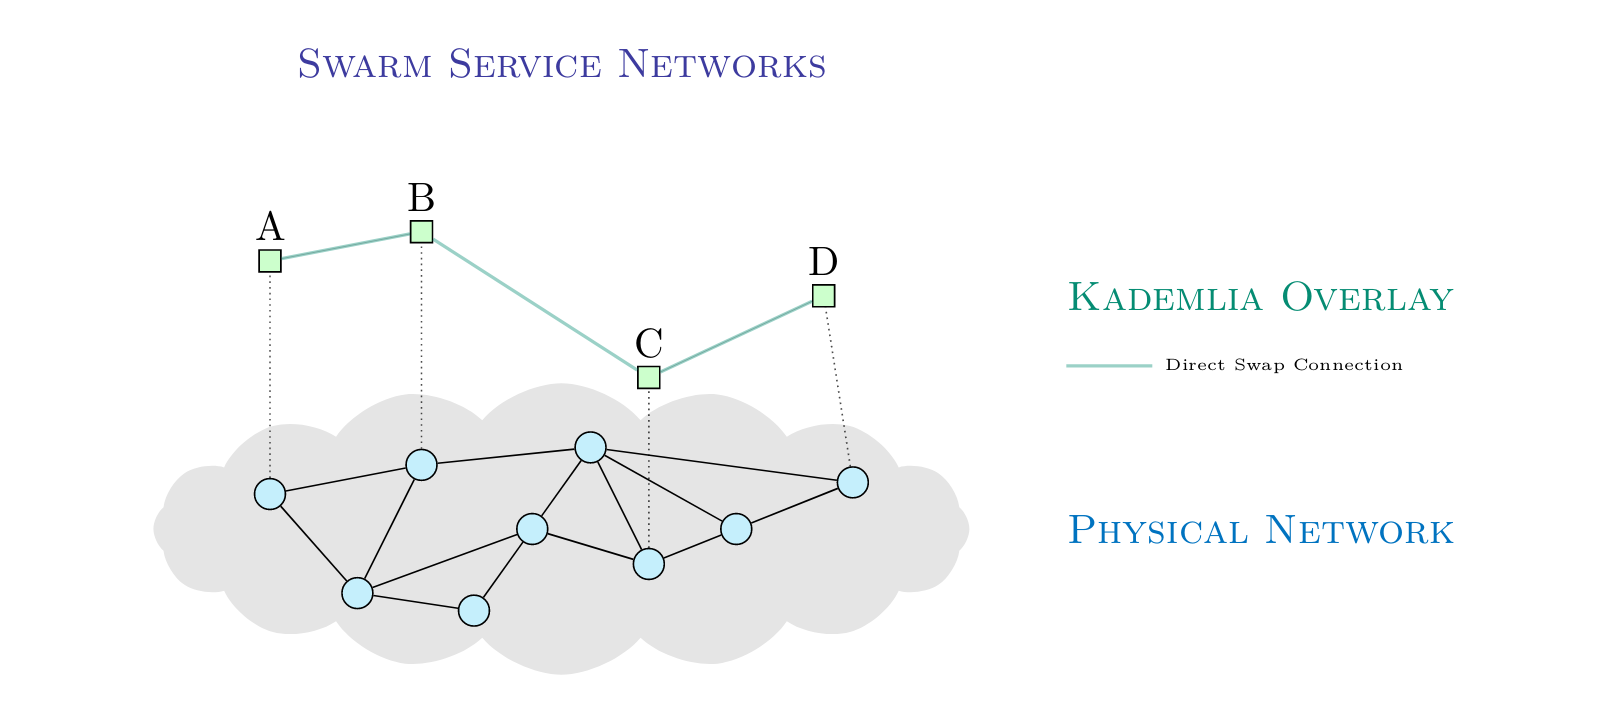
\includegraphics[width=\textwidth]{overlay-underlay.png}
\end{block}
\end{frame}

\begin{frame}{service networks}
  \begin{block}{swap channels}
    repeated dealings, limited peerset
  \end{block}
  \begin{block}{overlay topology}
    incentivised relaying, guaranteed routing
  \end{block}
  \begin{block}{swap channel networks}
    indirect transactions: ad-hoc one-off transaction between any two nodes
  \end{block}
  \begin{block}{warranted service provision networks}
    load-balanced tasks, instant service guarantee in a single swap: request and disappear, finger-pointing
  \end{block}
\end{frame}

\begin{frame}{indirect transactions}
\begin{block}{}
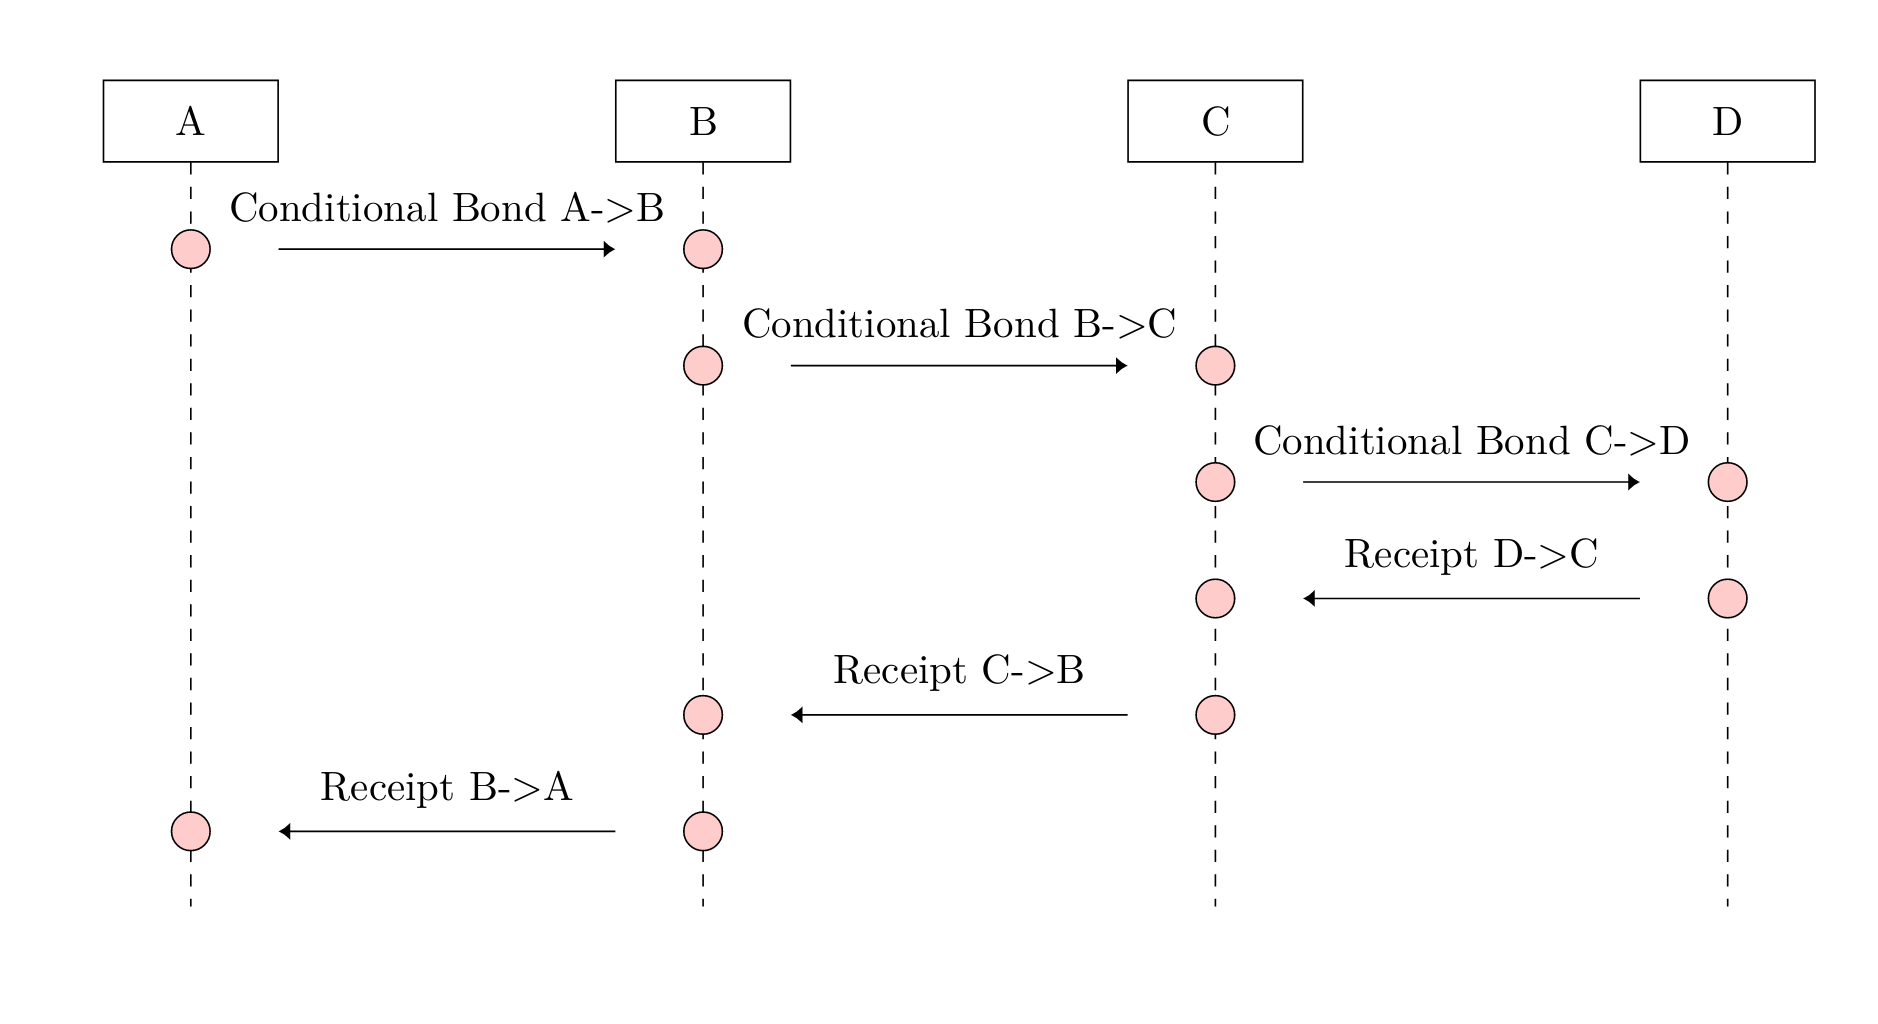
\includegraphics[width=\textwidth]{bond.png}
\end{block}
\end{frame}

\begin{frame}{service economy}
  \begin{block}{composition}
  \begin{itemize}
    \item reverse auction for competitive bounties
    \item atomic swap for exchange
  \end{itemize}
  \end{block}
  \begin{block}{example}
  \begin{itemize}
    \item crash proof of custody for storage insurance
    \item database insertion, indexing using pot escrow
    \item mailbox, chat history, persistent comments services
  \end{itemize}
  \end{block}
\end{frame}


\begin{frame}[plain]{contact and contribute}
\begin{block}{contact and contribute}
\begin{itemize}
\item swap swear and swindle working group and paper: \texttt{https://github.com/ethersphere/swarm/wiki/Working-groups}
\item swarm channel: \texttt{https://gitter.im/ethereum/swarm}
\item orange papers \texttt{http://swarm-gateways.net/}
\item join our research channel \texttt{https://gitter.im/ethersphere/orange-lounge}
\item twitter \texttt{https://twitter.com/ethersphere}
\end{itemize}
\end{block}

\end{frame}

\end{document}
